To introduce the \textbf{Fisher Information} (FI), we will start off with how it is defined and used in statistics.\\
Let's define a statistical model $f(x_i|\theta)$ that represents how a parameter $\theta$ is related to the outcomes $x_i$ of random variables $X_i$\cite{StatisticFisherInfoTutorial}. As an example of what this means, lets look at a Galton board. For readers that are not familiar with a what Galton boards are, there is an example photograph in \cref{fig:}. It's a famous mechanical model that shows binomial distributions, which are approximations of the normal distribution. If we place many balls at the top of the board and let them fall to the bottom, the amount of balls that end up in each cell are distributed according to the binomial distribution. 
\begin{figure}
	\centering
	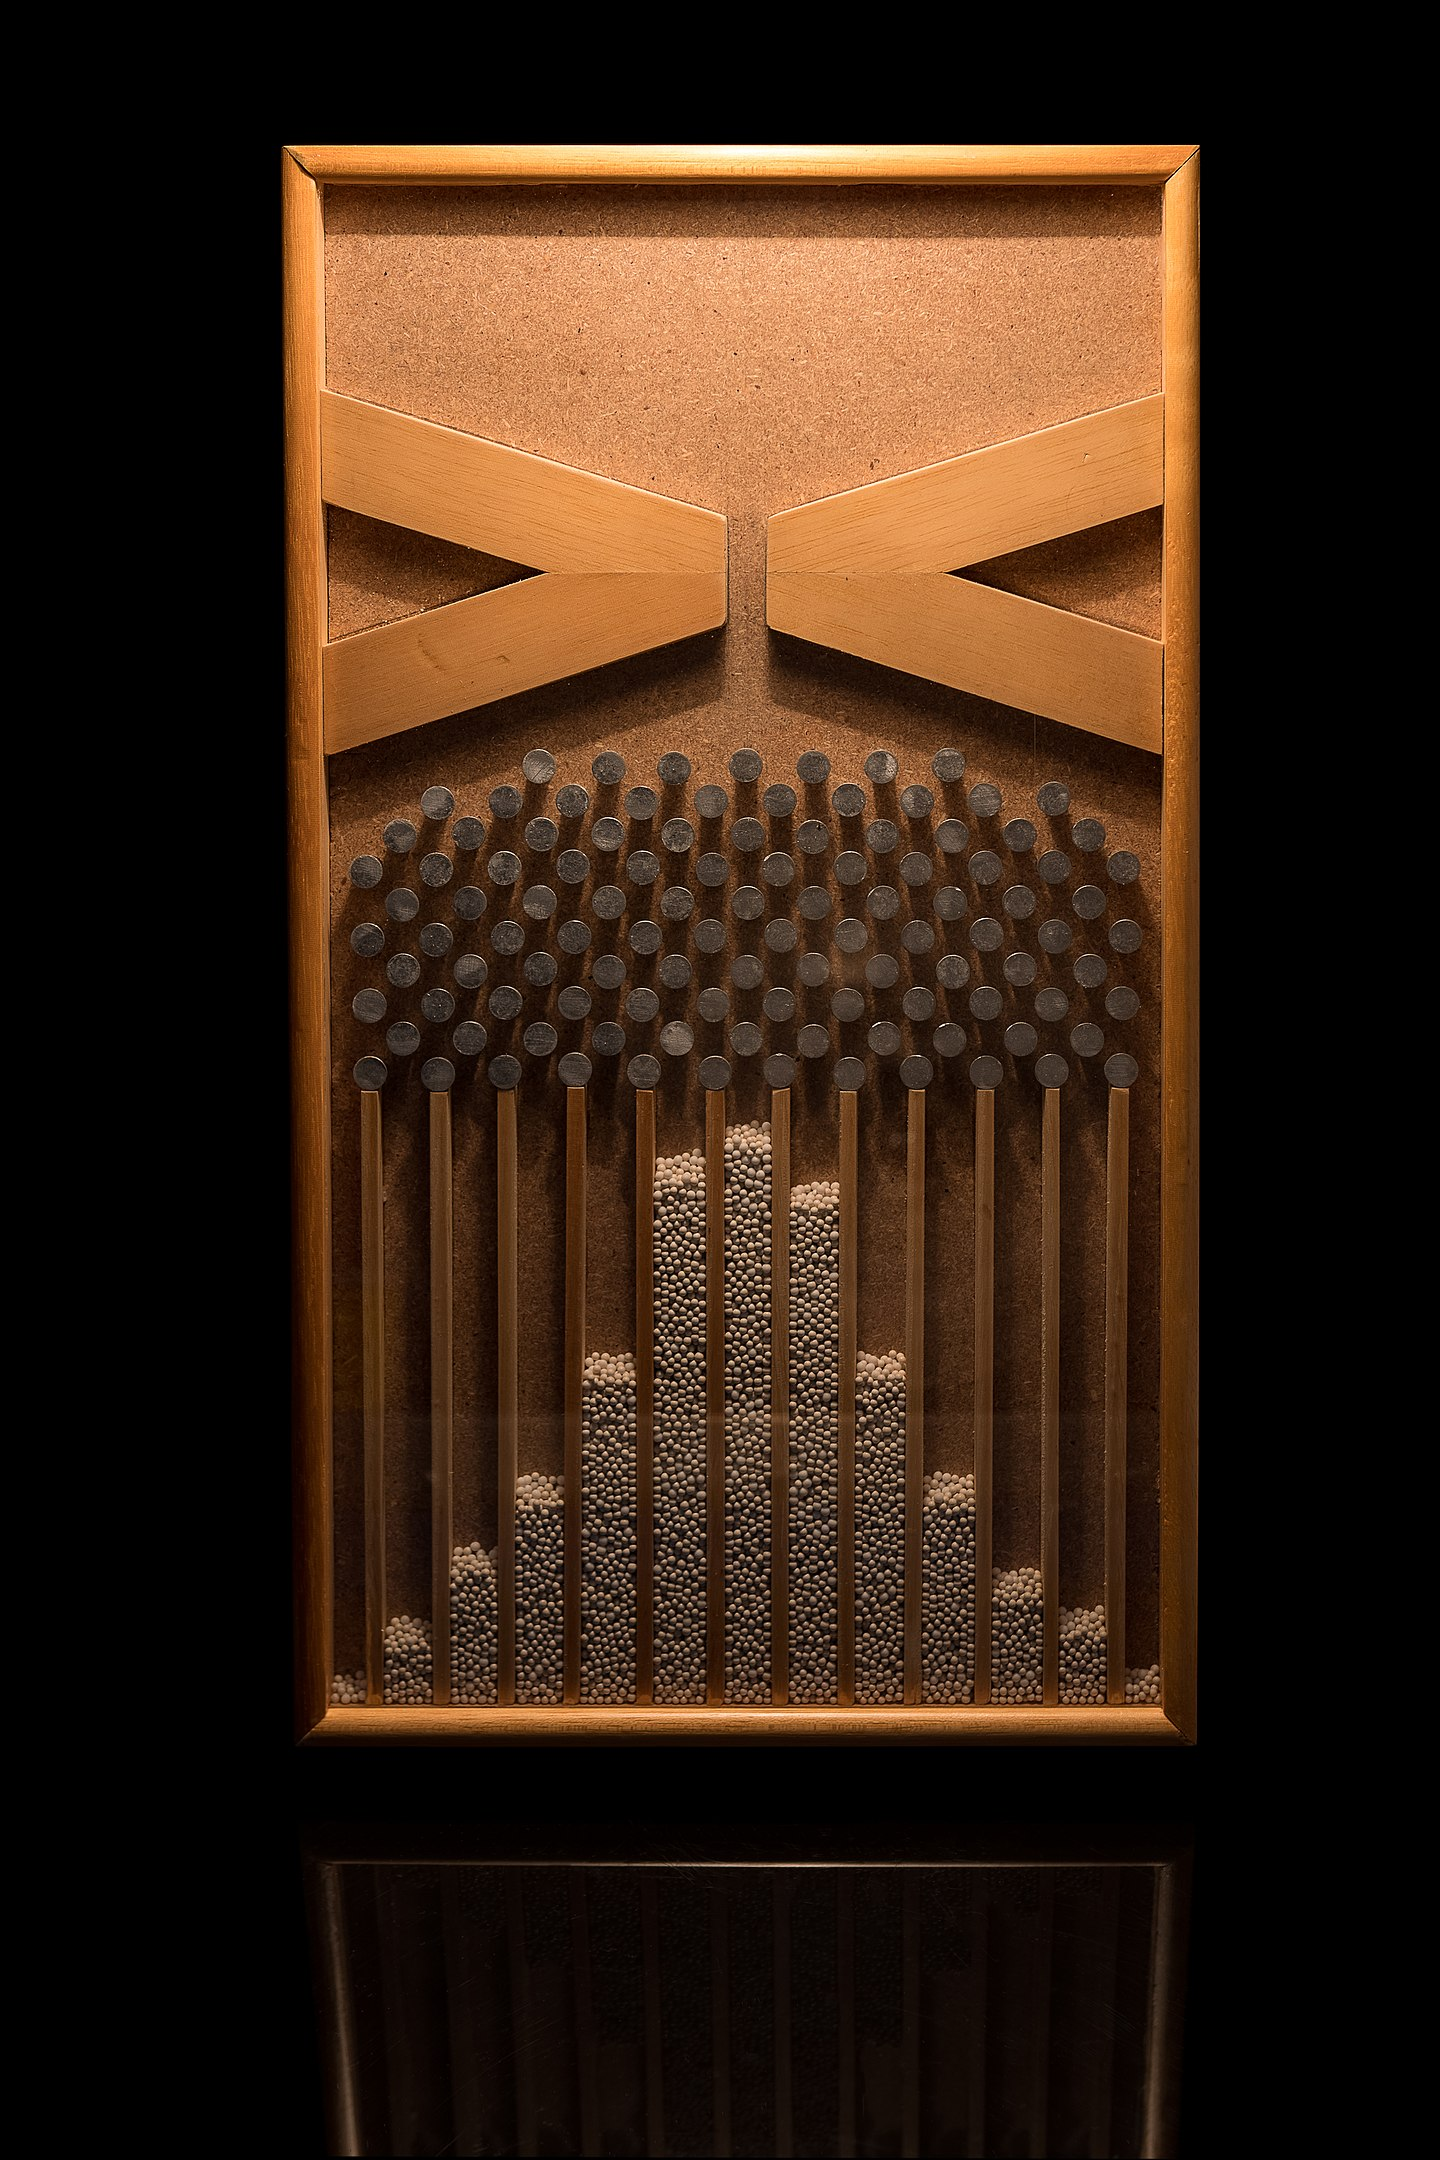
\includegraphics[width = 4cm]{text/FisherInformation/plots/GaltonBoard.jpg}
	\caption{This figure shows a picture of a Galton board. Taken from \cite{GaltonBoardPicture}.}
\end{figure}
Going back to the statistical model 
\begin{figure}
	\centering
	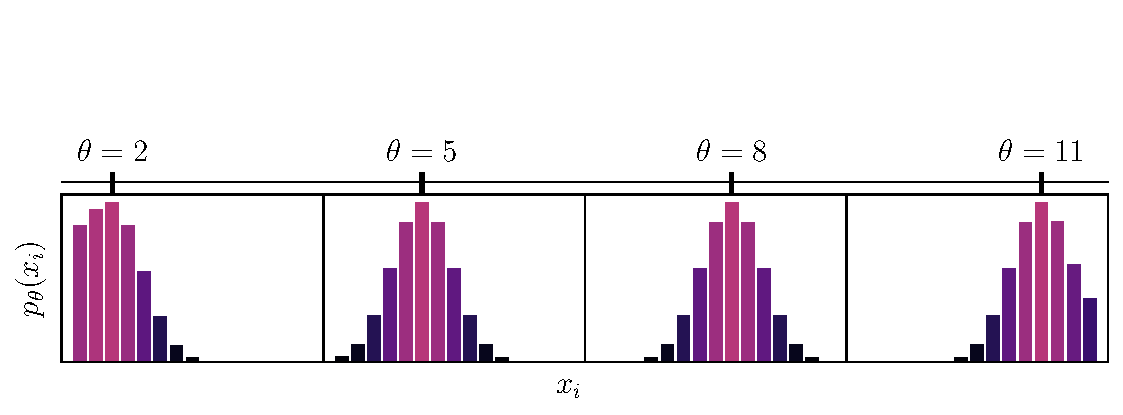
\includegraphics[width = \textwidth, clip, trim= 0cm 0cm 0cm 2.2cm]{text/FisherInformation/plots/GaltonDistributionsPlot.pdf}
	\caption{This figure shows a picture of a Galton board. Taken from \cite{fig:GaltonBoardPicture}.}
\end{figure}